% ============================================================
%  Projector-Side PE Audit — ICASSP 2027 Submission
%  Upload this directory as one Overleaf project; the method
%  figure is generated inline with TikZ.
% ============================================================
\documentclass{article}
\usepackage{spconf,amsmath,graphicx,hyperref}
\usepackage{amssymb}
\usepackage{booktabs,multirow,array,xcolor}
\usepackage{tikz}
\usetikzlibrary{arrows.meta,positioning,fit,backgrounds,calc}

% Title.
% ------
\title{REVISITING PROJECTOR-SIDE POSITIONAL ENCODING IN
       HIGH-RESOLUTION VISION--LANGUAGE MODELS}

% Authors and affiliations.
% -------------------------
\name{Guan-Jie Wang$^{1}$ \qquad
      Guan-Yan Yang$^{1}$ \qquad
      Farn Wang$^{1}$ \qquad
      Kuo-Hui Yeh$^{2}$}

\address{
$^{1}$ Department of Electrical Engineering,
National Taiwan University, Taipei, Taiwan\\
$^{2}$ National Yang Ming Chiao Tung University, Hsinchu, Taiwan\\
\{r12921107, f11921091, farn\}@ntu.edu.tw,
khyeh@nycu.edu.tw
}


\begin{document}
\maketitle

% ============================================================
\begin{abstract}
High-resolution vision--language models (VLMs) often add a
spatial positional encoding (PE) at the multimodal projector
even when the upstream vision path already preserves position.
We audit this term on VILA-HD-8B using five projector
conditions plus an initialization control, matched 312-step
cosine schedules, three seeds, and ten benchmarks.
Removing the projector PE yields 76.879$\pm$0.323\%.
The learned grid, its zero-initialized control, and uniform-polar
Fourier PE yield 76.847$\pm$0.123\%, 76.899$\pm$0.181\%, and
77.020$\pm$0.072\%, respectively.
The latter uses 0.46M rather than 2.61M PE parameters and needs
no grid interpolation. Separately, changing the learning-rate schedule horizon
from 1263 to 312 steps raises the same Cartesian-Fourier model
by 3.59 points on five OCR benchmarks. These results show that
upstream positional context and matched optimization protocol
are essential controls, while specialized projector PE choices
have small aggregate differences in this setting.
\end{abstract}
\begin{keywords}
positional encoding, VLM projector, Fourier features, ablation study, reproducibility
\end{keywords}

% ============================================================
\section{Introduction}

High-resolution VLMs use multi-scale processing, tiling, or
dynamic patch selection to preserve fine visual
detail~\cite{ps3,internvl,llava_hd}. A
vision encoder maps selected image regions to visual tokens,
and a multimodal projector maps these tokens into the language
model's embedding space. Positional information may enter at several stages: inside the
vision encoder, during selection-aware resampling, at the
projector, or through language-model position
IDs~\cite{ps3,mrope,v2pe}. Consequently, evaluating positional
encoding (PE) requires specifying both the intervention point
and the positional information retained elsewhere in the
architecture.

We study the marginal contribution of projector-side spatial PE
in the public PS3 path of VILA-HD-8B~\cite{ps3}. The
No-Projector-PE condition still retains upstream positional
information: PS3 resamples the vision encoder's positional
embedding and gathers it using the patch-selection map before
the projector. This motivates two controlled questions: how much
aggregate task performance is contributed by an
\emph{additional} projector spatial PE under this retained
positional pathway, and which compact representation provides
the best accuracy--parameter tradeoff when such a term is used?
We compare no additional projector spatial PE, a learned grid,
Cartesian Fourier features, selection-centered log-polar Fourier
features (LogRetina), and a PoPE-inspired uniform-polar Fourier
representation~\cite{pope_pe}.

Our contributions are:
\begin{enumerate}
  \item We audit the PS3 positional pathway and conduct a matched,
    three-seed comparison of five projector conditions plus a
    learned-grid initialization control. Their close aggregate
    results characterize the additional projector PE as a
    marginal component in this setting and establish retained
    upstream position as an essential control for interpreting
    projector-PE comparisons.

  \item Among the tested explicit PEs, uniform-polar Fourier
    achieves the highest observed ten-benchmark mean,
    77.020$\pm$0.072\%, while using 5.65$\times$ fewer PE
    parameters than the learned grid. The zero-initialized grid
    obtains 76.899$\pm$0.181\%; their +0.121-point mean
    difference changes sign across seeds, indicating
    comparable aggregate accuracy with substantially lower
    PE-module parameterization.

  \item Holding the Cartesian PE fixed, we measure a 3.59-point
    OCR-5 change at the same evaluated step across planned
    cosine-schedule horizons. This effect substantially exceeds
    the matched PE differences and establishes scheduler matching
    as an essential control for low-budget projector-PE
    comparisons.
\end{enumerate}

% ============================================================
\section{Related Work}

\noindent\textbf{Position in high-resolution VLMs.}
M-RoPE~\cite{mrope} decomposes position across temporal,
height, and width dimensions and is used by
Qwen2.5-VL~\cite{qwen25vl}; V2PE~\cite{v2pe}
studies smaller, variable visual-token position increments for
multimodal long contexts. PyPE~\cite{pype} instead changes the
ordering of visual position indices to mitigate long-range decay
in LLM-side RoPE. SliME~\cite{llava_hd} and
InternVL~\cite{internvl} provide high-resolution visual
processing strategies for multimodal models. These
methods operate on backbone or LLM-side positions; we isolate
the marginal contribution of an additive spatial term at the
projector while preserving the rest of the PS3 pathway.

\noindent\textbf{Spatial prompts and projector design.}
PIN~\cite{pin} learns a small spatial prompt inside a frozen VLM
to enable zero-shot object localization. Honeybee~\cite{honeybee}
redesigns the projector to preserve locality while controlling
the number of visual tokens. The public PS3/VILA-HD implementation~\cite{ps3}, by contrast,
combines prompt-aware selection with a learned
$729\times C$ spatial grid at the projector. We neither introduce localization supervision nor
replace the projector/token sampler; we ablate and replace only
this additional PS3 spatial term.

\noindent\textbf{Functional PE and necessity studies.}
Perceiver-VL~\cite{perceivervl} reports comparable performance with learned and Fourier PE for its latent array, providing a precedent for closely matched PE configurations in a different architecture. Functional PE generates position from coordinates
and avoids a resolution-indexed lookup table. Fourier mappings follow random
features~\cite{rahimi2007} and neural coordinate
encodings~\cite{tancik2020};
PoPE~\cite{pope_pe} instead decouples content and position in RoPE-based sequence models and is not a 2-D VLM-projector method. FlexiViT~\cite{flexivit}, NaViT~\cite{navit}, and
RoPE-ViT~\cite{ropevit} motivate spatial representations
that remain usable across varying patch sizes, image
resolutions, or aspect ratios.
Our distinct focus is a matched comparison among No-PE,
learned, and functional configurations after auditing position
already retained upstream.

% ============================================================
\section{Projector-Side Position Representations}

\begin{figure*}[t]
\centering
\resizebox{0.98\textwidth}{!}{%
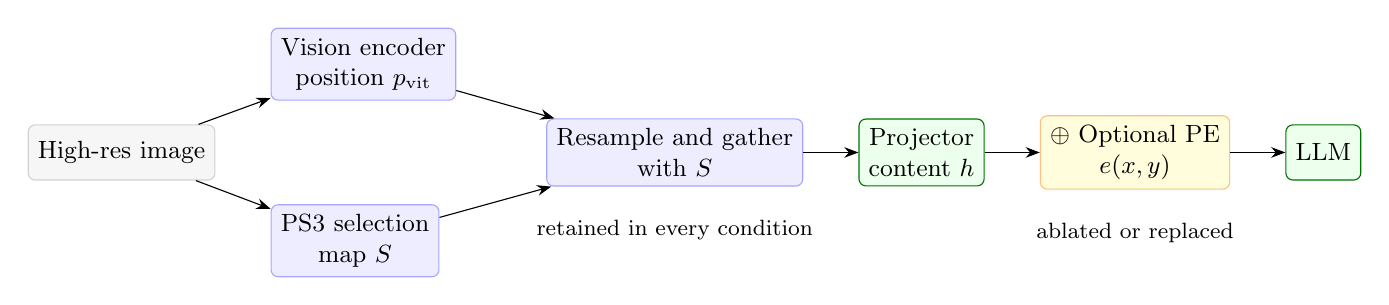
\begin{tikzpicture}[
  font=\small,
  box/.style={draw,rounded corners=2.5pt,minimum height=7mm,
              inner sep=3.5pt,align=center,fill=white},
  bluebox/.style={box,fill=blue!7,draw=blue!35},
  goldbox/.style={box,fill=yellow!14,draw=orange!50},
  greenbox/.style={box,fill=green!7,draw=green!45!black},
  graybox/.style={box,fill=gray!7,draw=gray!35},
  >={Stealth[length=1.8mm]},
  node distance=5mm and 9mm
]

\node[graybox] (img) {High-res image};
\node[bluebox,above right=3mm and 7mm of img] (vit)
  {Vision encoder\\position $p_{\rm vit}$};
\node[bluebox,below right=3mm and 7mm of img] (sel)
  {PS3 selection\\map $S$};
\node[bluebox,right=42mm of img] (gather) {Resample and gather\\with $S$};
\node[greenbox,right=7mm of gather] (proj) {Projector\\content $h$};
\node[goldbox,right=7mm of proj] (opt) {$\oplus$ Optional PE\\$e(x,y)$};
\node[greenbox,right=7mm of opt] (llm) {LLM};
\draw[->] (img) -- (vit);
\draw[->] (img) -- (sel);
\draw[->] (vit) -- (gather);
\draw[->] (sel) -- (gather);
\draw[->] (gather) -- (proj);
\draw[->] (proj) -- (opt);
\draw[->] (opt) -- (llm);
\node[below=3mm of gather,font=\footnotesize,align=center] (retained)
  {retained in every condition};
\node[below=3mm of opt,font=\footnotesize,align=center] (tested)
  {ablated or replaced};

\end{tikzpicture}
}

\caption{Audited positional pathway. PS3 resamples vision-encoder
position embeddings and gathers them with the selection map
before the projector. Our no-projector-PE condition removes only
the optional spatial term $e(x,y)$; upstream position and PS3
scale embeddings remain unchanged.}
\label{fig:overview}
\end{figure*}


For normalized global coordinates $(x,y)\in[-1,1]^2$, we test:
(i) no additional projector spatial PE;
(ii) a learned grid $P_{\rm grid}\in\mathbb{R}^{729\times C}$;
(iii) Cartesian Fourier PE; (iv) selection-centered log-polar
Fourier PE (LogRetina); and (v) uniform-polar Fourier PE.
The functional variants first map coordinates to $(u,v)$ and
then apply the same fixed Fourier basis and learned projection:
\begin{align}
 \phi(u,v)=\big[&\sin(2\pi2^ku),\cos(2\pi2^ku),\nonumber\\
                 &\sin(2\pi2^kv),\cos(2\pi2^kv)\big]_{k=0}^{K-1},\\
 e(x,y)&=W\phi(u,v)+b,\qquad W\in\mathbb{R}^{C\times4K}.
\end{align}
Cartesian uses $(u,v)=(x,y)$. Uniform polar uses normalized
radius and angle. LogRetina centers coordinates at the weighted
selection centroid $(\bar x,\bar y)$ and uses
\begin{equation}
 r'=\frac{\log(1+\alpha r)}{\log(1+\alpha)},\quad
 (u,v)=(r'\cos\theta,r'\sin\theta),
\end{equation}
with $\alpha=1$. With $K=32$ and $C=3584$, every functional
variant has $(4K+1)C=462{,}336$ learned parameters, versus
$729C=2{,}612{,}736$ for the grid: a 5.65$\times$ PE-module
reduction. Its parameter count is independent of the spatial
grid, so changing grid size does not require interpolating a
learned table. This reduction applies specifically to PE-module parameterization; end-to-end model size remains dominated by the 8B backbone.
Initialization is part of each tested configuration: standard Learned-Grid
PE is reinitialized from $\mathcal{N}(0,0.02^2)$, whereas the
new functional projection weights and biases are zero-initialized
so that they initially preserve the pretrained-model function.
We therefore also report a zero-initialized Learned-Grid control
(A0), which uses the identical training and evaluation protocol.
This diagnostic separates the initialization question from the
five primary configurations without replacing the standard grid
reference.
A separate sparse diagnostic additionally evaluates Fixed-Origin Log-Polar Fourier PE (internal code D); it is not a primary matched-table row.

% ============================================================
\section{Experiments}

\subsection{Setup}

All comparisons use the same VILA-HD-8B~\cite{ps3}
PS3-1.5K Stage-2 checkpoint, with a Qwen2-family 7B language
backbone and a SigLIP2 vision tower~\cite{siglip2}.
The ten benchmarks comprise five OCR tasks---TextVQA
\cite{textvqa}, DocVQA \cite{docvqa}, ChartQA \cite{chartqa},
OCRBench \cite{ocrbench}, and InfoVQA \cite{infovqa}---hereafter
denoted \textbf{OCR-5}; four spatial/grounding tasks---V*Bench
\cite{vstar}, MMBench \cite{mmbench}, GQA \cite{gqa}, and
POPE \cite{pope_bench}---and MathVista~\cite{mathvista}.
OCRBench uses the repository's normalized STVQA-style accuracy
for within-study comparison rather than an official leaderboard
score.
TextVQA uses its validation split, MathVista uses \texttt{testmini},
and GQA uses balanced test-dev. DocVQA and InfoVQA use ANLS;
ChartQA uses the repository's normalized exact/numeric-tolerance
accuracy, and the remaining tasks use their repository accuracy
evaluators. For each seed, OCR-5 and 10-benchmark results are
unweighted macro-averages of the corresponding percentage scores.

The 81k SFT mixture contains 12k each from ChartQA and DocVQA,
25k from ShareGPT4V~\cite{sharegpt4v},
24k from SVIT-Conv/CR~\cite{svit}, and 8k from
Tulu~\cite{tulu}.
All runs use effective batch size 64, LoRA~\cite{lora} rank
$r{=}64$ and scaling $\alpha{=}128$, 4-bit
QLoRA~\cite{qlora}, and one RTX~4090. A full-budget one-epoch
run takes approximately 43~h; the matched 312-step runs take
10.6--10.7~h according to their trainer states.

The primary comparison uses independent 312-step runs with the
same data mixture and seeded-sampler protocol, effective batch size 64, cosine
horizon, and seeds 42/1234/2024. Approximately one quarter of an
epoch is observed; this is a compute-budget condition, not a
fixed 25\% subset. We use formal method names in the paper;
internal experiment codes are N (No Projector Spatial PE), A
(Learned-Grid PE), A0 (zero-initialized Learned-Grid control), C
(Cartesian Fourier PE), E
(Selection-Centered Log-Polar Fourier PE), and F
(Uniform-Polar Fourier PE). The N condition zeros only the
additional spatial PE module; vision-encoder position and PS3
high/low-resolution scale embeddings are retained.

\textbf{Statistical scope:}
All five primary rows and the A0 diagnostic use matched exposure, schedule,
deterministic decoding, and token limits. Standard deviations
are sample SDs over the three predetermined seed-level macro-averages. With $n=3$,
we report observed means and paired differences rather than
population-level significance. The archived Cartesian
step-312 checkpoint from a 1263-step schedule appears only in
the separate scheduler control.

\subsection{Main Results}

\begin{table}[!t]
\centering
\caption{Matched 312-step results over three seeds (\%). A0 is
an initialization diagnostic; all rows share exposure, horizon,
and evaluation.}
\label{tab:main}
\setlength{\tabcolsep}{3.5pt}
\resizebox{\columnwidth}{!}{%
\begin{tabular}{lccc}
\toprule
Method & PE Params & OCR-5 & 10-benchmark \\
\midrule
No Projector Spatial PE & 0 & 77.020$\pm$0.105 & 76.879$\pm$0.323 \\
Learned-Grid PE & 2.61M & 76.570$\pm$0.352 & 76.847$\pm$0.123 \\
Learned-Grid PE, zero init (A0) & 2.61M & 76.833$\pm$0.197 & 76.899$\pm$0.181 \\
Cartesian Fourier PE & 0.46M & 76.696$\pm$0.044 & 76.893$\pm$0.128 \\
Selection-Centered Log-Polar PE & 0.46M & 76.759$\pm$0.254 & 76.901$\pm$0.150 \\
Uniform-Polar Fourier PE & 0.46M & \textbf{77.078$\pm$0.140} & \textbf{77.020$\pm$0.072} \\
\bottomrule
\end{tabular}
}
\end{table}

Table~\ref{tab:main} answers the necessity question first. No
Projector Spatial PE is within 0.032 points of Learned-Grid PE
and within 0.141 points of the best mean over ten benchmarks;
its paired ordering against Uniform-Polar Fourier reverses
across seeds. The tested system therefore characterizes the additional
projector spatial PE as a marginal component under the matched
setting, while the upstream positional pathway in Fig.~\ref{fig:overview} remains active.

Among explicit PEs, Uniform-Polar Fourier has the highest mean and lowest observed across-seed dispersion of the ten-benchmark macro-average. A0 differs from
the standard grid by only +0.052 points on average, with mixed
paired signs.
Uniform-Polar differs from A0 by +0.251, +0.284, and
$-0.171$ points for seeds 42, 1234, and 2024
(mean +0.121); the mixed paired signs characterize the
aggregate difference as small relative to seed variation.
Cartesian, LogRetina, and Uniform-Polar remain close, while all
functional variants use 5.65$\times$ fewer PE parameters than
the learned grid.


\subsection{Scheduler-Horizon Control}

\begin{table}[!t]
\centering
\caption{Same Cartesian Fourier PE evaluated at step 312 under
different cosine horizons; OCR-5 over three seeds (\%).}
\label{tab:robust}
\setlength{\tabcolsep}{4pt}
\small
\begin{tabular}{lccc}
\toprule
Condition & Seed scores & Mean & $\sigma$ \\
\midrule
Step 312 / horizon 1263 & 72.49/73.99/72.84 & 73.11 & 0.78 \\
Step 312 / horizon 312 & 76.70/76.74/76.65 & 76.70 & 0.04 \\
\bottomrule
\end{tabular}
\end{table}

The archived run and matched run use the same data mixture,
seeded-sampler protocol, model family, Cartesian PE, optimizer
hyperparameters, evaluated step, and seeds; the treatment is the
planned schedule horizon. Because the warmup ratio remains 0.03,
the absolute warmup also changes from 38 to 10 steps together
with the cosine trajectory. The logged
step-312 learning rates are $1.763\times10^{-5}$ and zero.
Changing the complete learning-rate schedule raises the mean by 3.59 points, much more
than any primary-table difference. A training fraction must
therefore specify both data exposure and scheduler horizon;
an intermediate checkpoint of a long schedule is not
equivalent to a completed short-budget run.

\subsection{Interpretation and Scope}

The close means indicate that coordinate-system choice has only
a small aggregate effect under the matched setting. LogRetina
also changes the origin using the selection centroid, so its
comparison with fixed-origin Cartesian and uniform-polar
encodings reflects complete configurations rather than an
isolated geometry intervention. In a separate one-round,
single-seed diagnostic, fixed- and dynamic-origin log-polar
variants obtain 75.8\% and 75.9\%, respectively, placing the
observed centroid effect within the narrow range seen among the
primary coordinate variants. Log compression therefore remains
a foveated design choice whose accuracy benefit may depend on
broader backbone, resolution, or training regimes.

\noindent\textbf{Scope and limitations.}
The controlled evaluation covers one VILA-HD-8B backbone and
three seeds, while the centroid diagnostic uses a single seed.
The demonstrated 5.65$\times$ reduction applies to PE-module
parameterization, which is small relative to the 8B model, and
does not establish end-to-end compression or latency gains.
Multi-backbone and cross-resolution evaluation provides
a natural next step for testing the generality of these findings.

% ============================================================
\section{Conclusion}

We audit the marginal contribution of projector-side spatial PE
in high-resolution VILA-HD-8B while retaining its upstream
selection-aware positional pathway. Across five primary
conditions and an initialization control, the three-seed
ten-benchmark means span only 0.173 points, characterizing the
additional projector PE as a marginal component in this setting.
Among the tested explicit PEs, Uniform-Polar Fourier achieves
the highest observed mean while using 5.65$\times$ fewer PE
parameters than the grid controls and avoiding grid-table
interpolation. Its mixed seed-level ordering relative to the
initialization-matched grid further characterizes their aggregate
accuracy as comparable.

The larger finding is methodological: changing the planned
cosine-schedule horizon moves the same Cartesian PE by 3.59
OCR-5 points, substantially more than the matched differences
among PE configurations. Reliable projector-PE comparisons
therefore require an explicit audit of retained upstream
positional information together with matched data exposure and
learning-rate scheduling. Under these controls, architectural
context and training protocol exert larger observed effects than
the tested coordinate refinements.

% ============================================================
% References + Acknowledgment (an optional fifth page may contain only these)
\section*{Acknowledgment}
The authors acknowledge the use of OpenAI ChatGPT and Codex for assistance with language editing and visualization-code development during manuscript preparation.

\bibliographystyle{IEEEbib}
{\small
\begin{thebibliography}{99}

\bibitem{ps3}
B.~Shi, B.~Li, H.~Cai, Y.~Lu, S.~Liu, M.~Pavone, J.~Kautz,
S.~Han, T.~Darrell, P.~Molchanov, and H.~Yin,
``Scaling vision pre-training to 4K resolution,''
in \emph{Proc.\ CVPR}, 2025, pp.~9631--9640.

\bibitem{internvl}
Z.~Chen et~al.,
``InternVL: Scaling up vision foundation models and aligning
for generic visual-linguistic tasks,''
in \emph{Proc.\ CVPR}, 2024, pp.~24185--24198.

\bibitem{llava_hd}
Y.-F.~Zhang, Q.~Wen, C.~Fu, X.~Wang, Z.~Zhang, L.~Wang, and
R.~Jin,
``Beyond LLaVA-HD: Diving into high-resolution large multimodal
models,''
\emph{arXiv:2406.08487}, 2024.

\bibitem{pope_pe}
A.~Gopalakrishnan, R.~Csord\'{a}s, J.~Schmidhuber, and
M.~C.~Mozer,
``Decoupling the `what' and `where' with polar coordinate
positional embeddings (PoPE),''
\emph{arXiv:2509.10534}, 2025.

\bibitem{qwen25vl}
S.~Bai et~al.,
``Qwen2.5-VL technical report,''
\emph{arXiv:2502.13923}, 2025.

\bibitem{mrope}
P.~Wang et~al.,
``Qwen2-VL: Enhancing vision-language model's perception of
the world at any resolution,''
\emph{arXiv:2409.12191}, 2024.

\bibitem{tancik2020}
M.~Tancik, P.~P. Srinivasan, B.~Mildenhall, S.~Fridovich-Keil,
N.~Raghavan, U.~Singhal, R.~Ramamoorthi, J.~T. Barron, and R.~Ng,
``Fourier features let networks learn high frequency functions
in low dimensional domains,''
in \emph{Proc.\ NeurIPS}, 2020.

\bibitem{rahimi2007}
A.~Rahimi and B.~Recht,
``Random features for large-scale kernel machines,''
in \emph{Proc.\ NeurIPS}, 2007.

\bibitem{ropevit}
B.~Heo, S.~Park, J.~Han, and S.~Yun,
``Rotary position embedding for vision transformer,''
in \emph{Proc.\ ECCV}, 2024.

\bibitem{v2pe}
J.~Ge et~al.,
``V2PE: Improving multimodal long-context capability of
vision-language models with variable visual position encoding,''
in \emph{Proc.\ ICCV}, 2025, pp.~21070--21084.

\bibitem{lora}
E.~J.~Hu, Y.~Shen, P.~Wallis, Z.~Allen-Zhu, Y.~Li, S.~Wang,
L.~Wang, and W.~Chen,
``LoRA: Low-rank adaptation of large language models,''
in \emph{Proc.\ ICLR}, 2022.

\bibitem{qlora}
T.~Dettmers, A.~Pagnoni, A.~Holtzman, and L.~Zettlemoyer,
``QLoRA: Efficient finetuning of quantized LLMs,''
in \emph{Proc.\ NeurIPS}, 2023.

\bibitem{siglip2}
M.~Tschannen et~al.,
``SigLIP 2: Multilingual vision-language encoders with improved
semantic understanding, localization, and dense features,''
\emph{arXiv:2502.14786}, 2025.

\bibitem{sharegpt4v}
L.~Chen et~al.,
``ShareGPT4V: Improving large multi-modal models with better
captions,''
in \emph{Proc.\ ECCV}, 2024, pp.~370--387.

\bibitem{svit}
B.~Zhao, B.~Wu, M.~He, and T.~Huang,
``SVIT: Scaling up visual instruction tuning,''
\emph{arXiv:2307.04087}, 2023.

\bibitem{tulu}
Y.~Wang et~al.,
``How far can camels go? Exploring the state of instruction
tuning on open resources,''
\emph{arXiv:2306.04751}, 2023.

\bibitem{infovqa}
M.~Mathew, K.~Bagal, R.~Tito, D.~Karatzas, E.~Valveny, and
C.~V.~Jawahar,
``InfographicVQA,''
in \emph{Proc.\ WACV}, 2022, pp.~1697--1706.

\bibitem{textvqa}
A.~Singh et~al.,
``Towards VQA models that can read,''
in \emph{Proc.\ CVPR}, 2019, pp.~8317--8326.

\bibitem{docvqa}
M.~Mathew, D.~Karatzas, and C.~V.~Jawahar,
``DocVQA: A dataset for VQA on document images,''
in \emph{Proc.\ WACV}, 2021, pp.~2200--2209.

\bibitem{chartqa}
A.~Masry, D.~X.~Long, J.~Q.~Tan, S.~Joty, and E.~Hoque,
``ChartQA: A benchmark for question answering about charts
with visual and logical reasoning,''
in \emph{Findings of ACL}, 2022, pp.~2263--2279.

\bibitem{ocrbench}
Y.~Liu et~al.,
``OCRBench: On the hidden mystery of OCR in large multimodal
models,''
\emph{Sci. China Inf. Sci.}, vol.~67, no.~12, art.~220102,
2024.

\bibitem{mathvista}
P.~Lu et~al.,
``MathVista: Evaluating mathematical reasoning of foundation
models in visual contexts,''
in \emph{Proc.\ ICLR}, 2024.

\bibitem{vstar}
P.~Wu and S.~Xie,
``V*: Guided visual search as a core mechanism in multimodal
LLMs,''
in \emph{Proc.\ CVPR}, 2024, pp.~13084--13094.

\bibitem{pope_bench}
Y.~Li et~al.,
``Evaluating object hallucination in large vision-language
models,''
in \emph{Proc.\ EMNLP}, 2023, pp.~292--305.

\bibitem{mmbench}
Y.~Liu et~al.,
``MMBench: Is your multi-modal model an all-around player?''
in \emph{Proc.\ ECCV}, 2024, pp.~216--233.

\bibitem{gqa}
D.~A.~Hudson and C.~D.~Manning,
``GQA: A new dataset for real-world visual reasoning and
compositional question answering,''
in \emph{Proc.\ CVPR}, 2019, pp.~6700--6709.

\bibitem{flexivit}
L.~Beyer, P.~Izmailov, A.~Kolesnikov, M.~Caron, S.~Kornblith,
X.~Zhai, M.~Minderer, M.~Tschannen, I.~Alabdulmohsin, and
F.~Pavetic,
``FlexiViT: One model for all patch sizes,''
in \emph{Proc.\ CVPR}, 2023, pp.~14496--14506.

\bibitem{navit}
M.~Dehghani et~al.,
``Patch n' Pack: NaViT, a vision transformer for any aspect
ratio and resolution,''
in \emph{Proc.\ NeurIPS}, 2023.

\bibitem{pype}
Z.~Chen, M.~Li, Z.~Chen, N.~Du, X.~Li, and Y.~Zou,
``Advancing general multimodal capability of vision-language
models with pyramid-descent visual position encoding,''
in \emph{Findings of ACL}, 2025, pp.~6324--6341.

\bibitem{pin}
M.~Dorkenwald, N.~Barazani, C.~G.~M. Snoek, and Y.~M. Asano,
``PIN: Positional insert unlocks object localisation abilities
in VLMs,''
in \emph{Proc.\ CVPR}, 2024, pp.~13548--13558.

\bibitem{honeybee}
J.~Cha, W.~Kang, J.~Mun, and B.~Roh,
``Honeybee: Locality-enhanced projector for multimodal LLM,''
in \emph{Proc.\ CVPR}, 2024, pp.~13817--13827.

\bibitem{perceivervl}
Z.~Tang, J.~Cho, J.~Lei, and M.~Bansal,
``Perceiver-VL: Efficient vision-and-language modeling with
iterative latent attention,''
in \emph{Proc.\ WACV}, 2023, pp.~4410--4420.

\end{thebibliography}
}

\end{document}
